\chapter{Introduction}  \label{chap:intro}

The standard Big Bang model of our universe shows that less than 5\% \citep{planck_collaboration_planck_2020} of the total energy density of the universe is in the form of baryons. All the `ordinary' matter which we see around us is made up of these baryons. Astronomers are interested in studying the distribution of these baryons to understand the evolution of the universe, formation of large scale structures. So, understanding this component of the universe is crucial for our comprehension of the cosmos.

\section{Where are the baryons ?}

While attempting the census of the baryons in the present universe, i.e at $z \sim 0$, cosmologists found that there is a shortfall from the total number obtained from the observations of Cosmic Microwave Background (CMB) and light element abundances predicted from big bang nucleosynthesis. In their study, \citet{Fukugita-1998} were able to account for about half of the expected number of baryons. Using cosmological simulations, \citet{cen-ostriker-1999} also argued that about 50\% of the baryons are yet to be detected. With time the surveys got better, however, recent surveys still show a deficit of $\sim 30$\% \citep{Shull}. This came to be known as the ``Missing Baryon Problem" at low redshift. At high redshift ($z>3$), nearly all the baryons have been accounted for, with around 3\% being collapsed in stars and galaxies and remaining $\sim97$\% are found in cool ($\sim10^4$ K) photo-ionised gas phase in the form of Ly$\alpha$ forests in intergalactic medium (IGM). 

Figure \ref{fig:Baryon-budget} shows the distribution of baryons at low redshift. Only less than 20\% of the baryons are in the form of collapsed structures in galaxies, circumgalactic medium (CGM), intercluster medium (ICM) and in cold gas (\ion{H}{i} and \ion{He}{i}). Rest of the 80\% baryons are in diffused IGM, mainly in two phases, around 30\% in cool photoionised phase observed through Ly$\alpha$ forests \citep{Danforth_2008,tilton_2012} and remaining 50\% are expected to be in Warm Hot Intergalactic Medium (WHIM). Out of these 50\%, nearly 20\% have been accounted mainly from the observations of Broad Lyman-$\alpha$ Absorbers (BLAs) (see section \ref{sec:WHIM-BLA}) and studies of \ion{O}{vi} absorbers \citep{Danforth_2008,tilton_2012,Tripp_2008,savage-2014}. WHIM can also be traced by X-ray absorbers at temperatures above $10^6$ K, by highly ionised species like \ion{O}{vii-viii}, \ion{Ne}{viii-x}, etc. However very few studies of such systems have been carried out because of unavailability of good X-ray data as these are very weak absorbers and are below the detection limits of current X-ray spectrographs \citep{yao_2012} (see section \ref{sec:WHIM-detection} for more details on detection of WHIM) . And remaining $\sim$ 30\% are missing from the observations. We will describe BLAs in detail in section \ref{sec:WHIM-BLA} as they we will be our `lamps' in finding the baryons in WHIM. 

Cosmological simulations \citep{cen-ostriker-1999,cen-ostriker-2006} shows that these `missing' baryons are residing in WHIM which has very low densities ($10^{-6}-10^{-4}$ cm$^{-3}$) and high temperatures ($10^5-10^7$ K). Simulations also show that WHIM is mainly formed via shock-heating of the in-falling gas from the IGM on the large scale structures. Because of its low density and temperature not high enough to emit in X-rays, it doesn't emit detectable amount of radiation to be observed in emission. And because of high temperatures, the gas is too collisionally ionised to imprint significant absorption signatures in the spectra of the background objects. Because of these difficulties much of the WHIM is yet to be detected. 

\begin{figure}[!t]
    \centering
    \vspace{5mm}
    \hspace{12mm}
    \includegraphics[width=0.75\linewidth]{Figures/Baryon-census.png}
    \caption{Baryon budget at low redshift universe ($z\sim0$). Credits : \citet{Shull}}
    \label{fig:Baryon-budget}
\end{figure}

\section{Detecting WHIM} \label{sec:WHIM-detection}

As discussed in previous section that around 50\% of the baryons are expected to be in WHIM, so in this section we describe how we can detect WHIM.

The WHIM is mainly detected with the help of quasars. The quasars are very bright sources of light, providing us an excellent source of background light. The matter in the intervening space between us and these quasars can leave absorption features in the spectra of these quasars, enabling us to `look' at this matter as shown in figure \ref{fig:qso-absorption}. It shows the absorption from the gas in IGM, marked as red lines, from different intermediate redshifts, whereas green marked lines are galactic absorption lines. The WHIM can be traced by highly ionised species like \ion{O}{vi-viii}, \ion{Ne}{viii-x}, etc. as these arise in high temperature gas phase \citep{tepper-2013}. Apart from high temperature gas these lines can also arise from photoionised gas phases. There are instances in the literature where the origin of these lines is uncertain, i.e whether they are coming from collisionally ionised or photoionised phase. For example, in their study of ionisation mechanisms of \ion{Ne}{viii}, \citet{Hussain-2017} found that the observed column densities of \ion{Ne}{viii} and \ion{O}{vi} can be explained by using the photoionisation models which also solves the problem of cooling in collisional ionisation at the predicted metallicities.   

So detecting these lines doesn't assure that we they are probing WHIM. Nevertheless, unavailability of high S/N X-ray data also makes it difficult to study WHIM using these lines. 
\\\\
Because of high temperatures of WHIM, the absorption lines can get thermally broadened. So detecting such broad features can show possibility of tracing high temperature gas phase. This gives us an another way of probing WHIM by using Broad Ly$\alpha$ Absorbers (BLAs) which we describe in the next section.

\begin{figure}
    \centering
    \includegraphics[width=\linewidth]{Figures/spec slice.png}
    \caption{Slice of spectrum of quasar HE0153-4520 ($z_{em}=0.4510$). Credits : \citet{danforth-2016}}
    \label{fig:qso-absorption}
\end{figure}


\section{Detecting WHIM using BLAs} \label{sec:WHIM-BLA}

Any Ly$\alpha$ absorption line with Doppler parameter (\emph{b}) $\gtrsim$ 40-45 km $\text{s}^{-1}$ can be loosely called a BLA. These $b$ values corresponds to temperatures of $9.7\times 10^4 - 1.2 \times 10^5$ K assuming a complete thermal broadening. BLAs are expected to host significant fraction of the baryons in the low-redshift universe \citep{Richter-2004,Richter-2006,Lehner-2006,Lehner-2007}. In spite of low neutral fraction of \ion{H}{i}, these lines can be detected up-to the temperatures of $\sim10^6$ K because of large abundance of Hydrogen. As these features are broad they are very shallow as compared to their narrower counterpart with same line strength. Thus high S/N data is required to detect BLAs. Detecting a BLA ensures that we are tracing WHIM. If a BLA is detected, then we can expect to see other highly ionised species as well. 

However, several narrow components can also blend together resulting in broad features. Figure \ref{fig:BLA} shows such an example. The left panel shows the broad line and second panel shows the fitted profile with multiple components to the line. The red shaded region is the contribution from BLA and rest is the contribution of narrower components. So, a careful modelling has to be done for such absorbers. If we find a candidate BLA in such features then we need to show that the other kinematically concurrent species are arising from a collisionally ionised gas phase as is the case of WHIM. To do so, we need to model the ionisation conditions prevalent in the absorber cloud which we describe in chapter \ref{chap:Ion-Model} in detail.

\begin{figure}[!h]
    \centering
    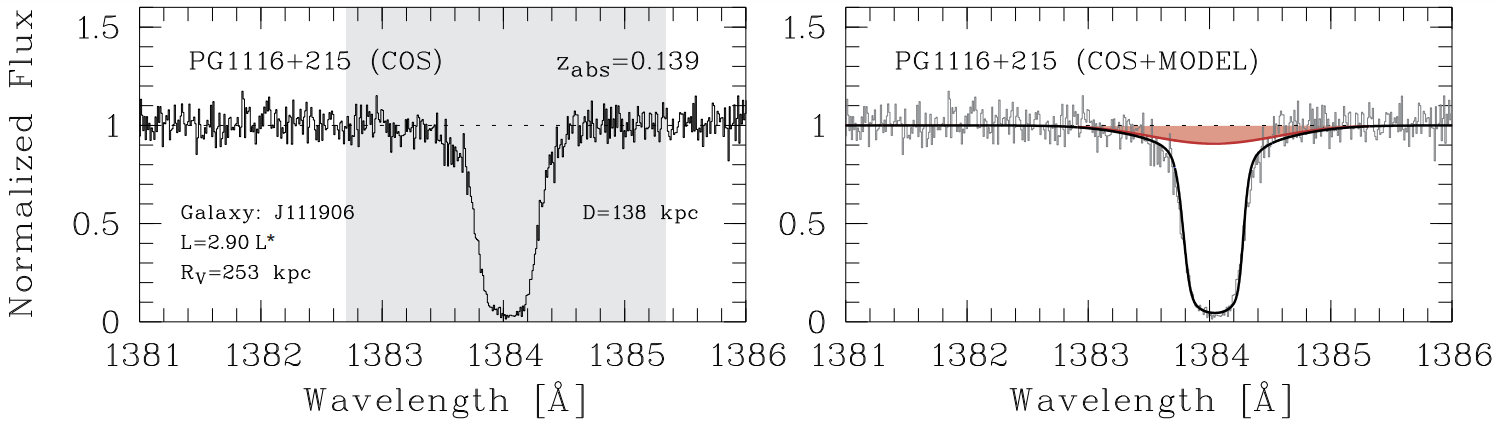
\includegraphics[width=\linewidth]{Figures/BLA.png}
    \caption{A BLA blended with other Ly$\alpha$ absorption lines towards the LOS of quasar PG1116+215 $(z_{em} = 0.176)$. Credits : \citet{Richter_2020}}
    \label{fig:BLA}
\end{figure}

There have been studies of BLAs on small scales but as these are difficult to observe they show varying results. For instance, \citet{Lehner-2007} have studied 7 AGN lines of sight to search for BLA candidates and estimated that BLAs contribute around 20\% to the total baryonic energy density ($\Omega_b$). However, a study by \citet{Danforth_2010}, which also studied 7 AGN lines of sight, report different results. They estimate the contribution of BLAs to be around 14\% in ($\Omega_b$).

So, there is a need to do a large survey of these BLAs to realise the abundance of baryons in these cosmic reservoirs. 

\section{Road-map for the Current Project}

In the current project we will be addressing the missing baryon problem with the help of BLAs. Currently, literature lacks comprehensive surveys of the BLAs on large datasets. So we will be doing a large survey of BLAs with high S/N HST/COS data. We will be doing Voigt profile measurements and will also model the ionisation conditions in the BLAs to infer their ionisation states. We will tehn results from this survey to  estimate the baryon content in BLAs and their  contribution to the total cosmic baryonic inventory ($\Omega_b$). 

The outline of this thesis is as follows : In chapter \ref{chap:data}, we describe the data which we will be using for our survey of BLAs. In chapter \ref{chap:VPFIT} we mention our Voigt profile fitting routine. Chapter \ref{chap:Ion-Model} describes the ionisation modelling of the absorbers and the method used for modelling. In chapter \ref{ch:PG0003}, we study a BLA candidate absorber system towards the LOS of quasar PG 0003+158 to test our methods. Chapter \ref{ch:Survey} describes our methodlogy for the survey, survey statisitics and overall results from the surevey. We discus the estimation of $\Omega_b(\text{BLA})$ in chapter \ref{ch:Omega-b} and we conclude by the summarising the current work and directions for future work in chapter \ref{ch:conclusions}. 
